% http://latex-cookbook.net/cookbook/examples/3d-plot/
\documentclass{standalone}
\usepackage{pgfplots}
\begin{document}
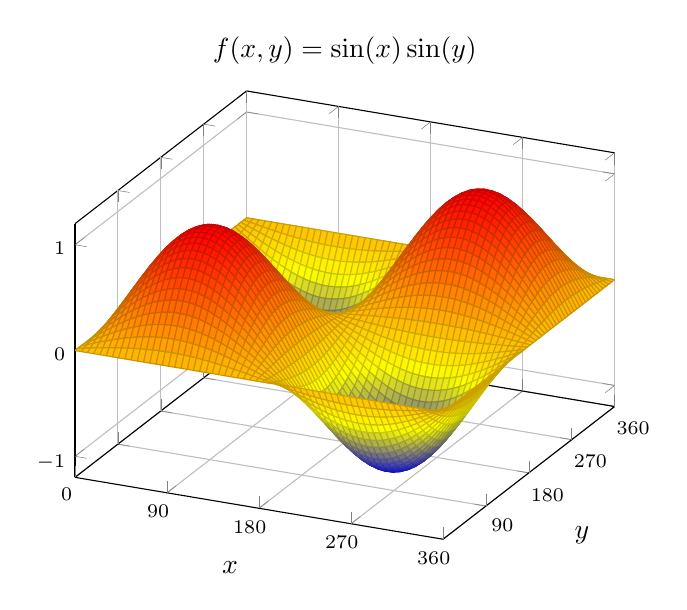
\begin{tikzpicture}
\begin{axis} [
    title = {$f(x,y) = \sin(x)\sin(y)$},
    xtick = {0,90,...,360},
    ytick = {90,180,...,360},
    xlabel = $x$, ylabel = $y$,
    ticklabel style = {font = \scriptsize},
	grid
]
\addplot3 [surf, domain=0:360, samples=60] 
	{ sin(x)*sin(y) };
\end{axis}
\end{tikzpicture}
\end{document}